\section{Beginning the project}

Being new to Javascript, the first few weeks of coding was learning the language and becoming familiar with how it all worked. This included knitting javascript together with HTML and CSS.

For any software project, keeping a good record of progress is important. In this case, GitHub was chosen as the version control. GitHub was simple to set up and use. It is used to keep notes of all of the progess of the project as it goes along and so advancements in the software can be documented easily, all in one place. It is also incredibly useful if changes are made to the software meaning that it no longer works. It is straightforward to revert to a previous commited version and carry on again from then.

Learning how to use the HTML 5 canvas as well as the methods associated with this that were available took some getting used to. The first mini project that I created was a small game that was played on a HTML canvas. The user would use a button to create numbers. They could drag and drop these numbers on top of each other. If they dragged an item over the top half of another item then the two numbers would subtract from each other and if over the bottom, then the two numbers would subtract.

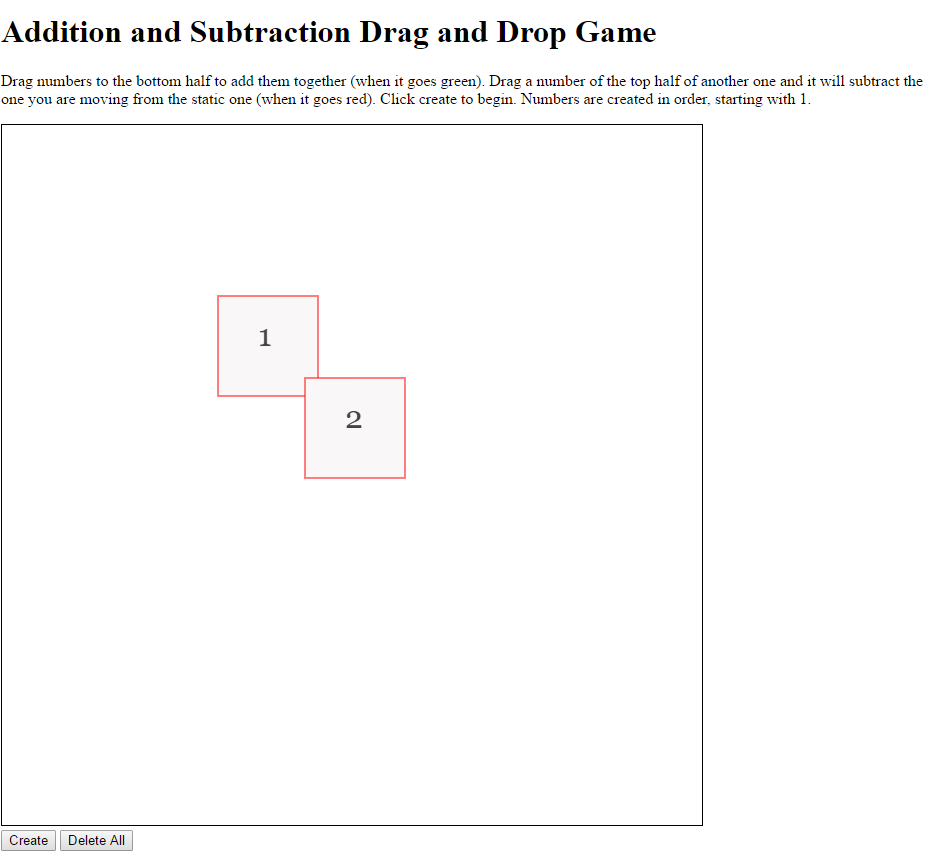
\includegraphics[scale=0.5]{addition1}

This game may sound trivial, but it helped me to understand how drag and drop worked, as well as understanding how items can react differently on a screen depending where the mouse is released. Most of this code is carried forward and used in the main Natural Deduction game.

\section{Drag and Drop}

Because I had no idea how to implement a drag and drop system, I followed an online tutorial and expanded my ideas from these foundations. http://html5.litten.com/how-to-drag-and-drop-on-an-html5-canvas/ This was the tutorial that was used for both the initial addition game and also for the main software project.

The three functions created in drag and drop are all event based. These are when the mouse is clicked down, when the mouse is moved and when the mouse is released. All three functions have important roles and do different jobs that make the drag and drop successful.

When the mouse is pressed down, an event handler runs, which runs a function. The function iterates through all of the objects on screen, seeing if the location of the mouse click is in the same position as any of the objects. If this is the case then a variable is set which says that an element needs to be moved. The moving mouse function 'myMove' is always executed, but the logic within it is only run when an object on the screen is selected to drag and drop because the variable is set. The logic within the moving function went through different phases of development as the project progressed. Explained in detail below is both the legacy system and the new, improved way that it now works.

\subsection{Original Colour System}

When implementing the move function in the software, thought had to be given to how the system would react when items were dragged on top of each other. Original thinking was to base what happened to objects based on the location of other objects. Because of the tree structure, it naturally splits into four different parts. Top left, bottom left, top right and bottom right are all possible locations where a part of a proof can be located. The original system worked out the location of all the objects on the screen. If another object was dragged over one of the objects, then depending which corner it was dragged over, the algorithm will set the borders of the two objects of a certain colour. Different colours would be set depending on what type of object is being highlighted. 

Variables and conditionals can be dragged onto by other objects of the same type. In the figures below, dragging to the conjunction onto the right hand side of the 'A' lights up both of the objects' borders red. Dragging the conjunction to the left hand side of the 'A' lights both of the borders green.
 
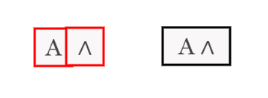
\includegraphics[scale=0.75]{AConjunction}
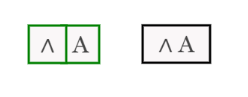
\includegraphics[scale=0.75]{ConjunctionA}

The same logic applies to proof structures as shown in the figure below, but all four of the corners could be dragged over to give different coloured bordered. Releasing the mouse when the borders are highlighted removes the object that is being dragged and places whatever is on the moving object to the static element in the correct corner.  

\centerline{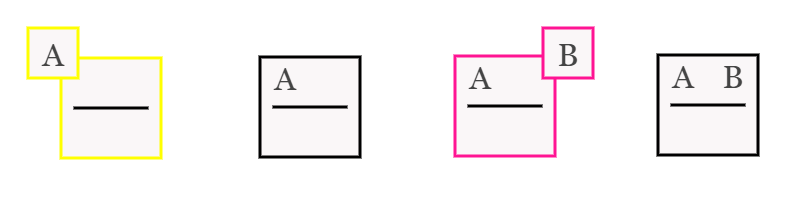
\includegraphics[scale=0.7]{oldColour}}

This makes it clear which part of the proof the user is dragging to. This is the advantage of this method. Colours makes it clearer to the user and it means once a user is familiar with it, they will know what to do in future. This is also a disadvantage because it does not come across as intuitive because the colours are unknown to the user before they start the game. There are also no obvious points on the proof where the user can drag to, and without any kind of prompt it can be difficult about the possible valid moves available.

Another issue occurs when multiple layers of proof are dragged together. This system of associating colours with the area user drags to does not work intuitively when building proofs. Natural deduction proofs are often built from the bottom up. With this method, proofs cannot be built from bottom up because the dragging and dropping is all associated with the first object that is dragged onto. Any new proof dragged onto the top left or top right of the proof will remove the existing structure that is there. This leads to a peculiar way of forming proofs of multiple layers. Because of these reasons and reacting to feedback echoing this, the way users dragged onto objects was changed.  

\subsection{Dots System}

A redesign of the system made the software fulfil more of the initial requirements, so it was a positive step, even if it was more technically more difficult. The idea behind this was to make it clearer to the user what moves were valid. The goal of the new system was also to provide a more flexible way of creating proofs, where users could drag onto any part of proof that was missing. This was achieved by adding dots to the proof structure.

Dots automatically show to the user where they can drag onto on the proof. It makes it much clearer visually and it is more intuitive. Because now every dot in the proofs could be dragged onto, locations of each dot needed to be stored. This meant that every dot had to be a seperate object with its own unique ID number and location information. These ID numbers would link to every proof object, so each proof object that can be dragged and dropped knows which dots are associated with it.

Also in the dot object is the colour of the border. If one of the objects is dragged over the location of the dot, then both the dot and the object being dragged over will turn purple. This is to let the user know which elements are being hightlighted and what is going to happen if the user releases the mouse. This is a great improvement on the previous system and will reduce errors from the user because it is less likely that the user will make mistakes.  

\centerline{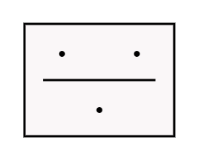
\includegraphics[scale=0.5]{dots}}

Another improvement from the first iteration of the code is that this system is more natural in the way proofs are created. Proof structures can be dragged onto the dots at the top of the current structure which leads to building a proof from bottom up. This is the conventional way to create Natural Deduction proofs in the tree structure and will offer a more realistic experience to the user.

In this way of dragging and dropping, the border of the object does not light up when the user is dragged onto. Only the dot of the static object lights up. Dragging to any corner of the object no longer has any effect, it is all based on where the dots are located. Because of this, multiple layers of proof can be built up with lots of dots contained in them. The user can then individually drop variables or statements onto the dots. This was something that was not possible in the previous way of dragging and dropping.

\centerline{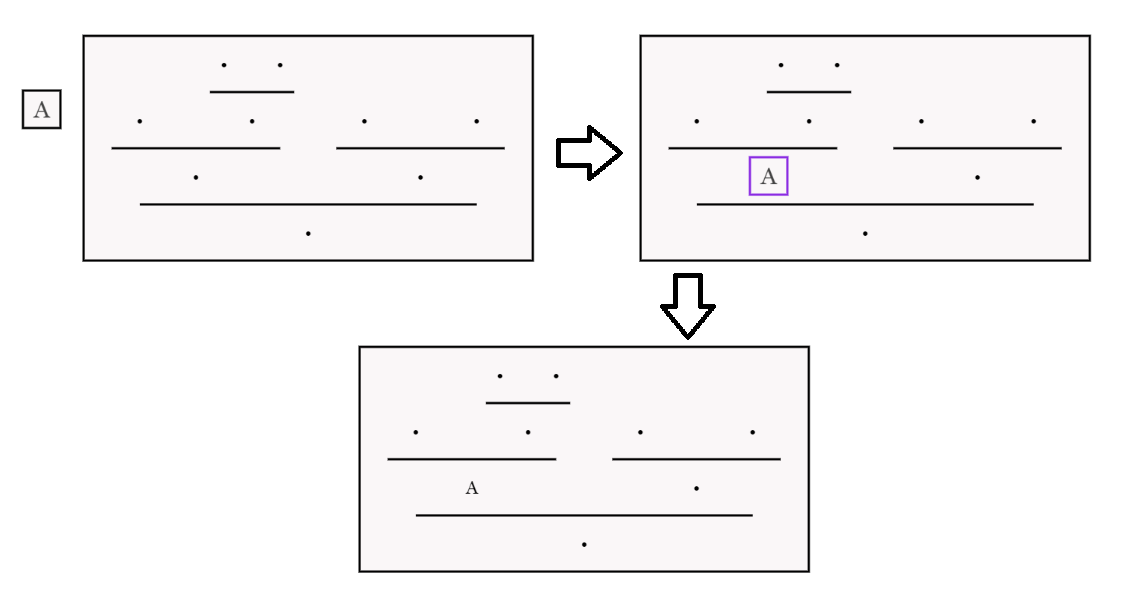
\includegraphics[scale=0.5]{dotsdnd}}

When another structure is placed on top of a dot, the dot object is removed and replaced with the structure that the moving object has, whether that is another proof structure or a statement. This structure of dragging and dropping proofs solved both of the main issues encounted in the original colour system. This is based on continuous internal testing as well as constant dialog with interested stakeholders such as the project supervisor Willem. Constant testing and improvement is a key part of any software project and will be covered in further detail later.  

\section{Data Structures}

Due to the visual representation of the proofs as trees, storing the data in a similar way made sense as it made it scalable. Basic objects are stored as a list. Each draggable object structure was the same, whether it was a proof structure or a variable. The core structure had four elements. The first element represented the top left corner, the second element represented the top right corner and the third and forth elements represented the bottom left and right corners respectively.

If an object was just a statement, like a variable, connector or a mixure of these, the string representing the statement would be placed in the first element and the remaining three elements would contain ``\%". A percentage string was one that let the program know that this element will never need to be used for this part of the proof. For the statement A $\wedge$  B, the data structure would be represented as [``A $\wedge$  B", ``\%", ``\%", ``\%"].

These percentage strings were also used for determining the layout of a tree structure. Two elements on the top and one on the bottom is used as well as one element on the top and one on the bottom in this game and they are represented with the following data structures:

\begin{center}
\begin{tabular}{ |c|c|c| } 
\hline
2 Top / 1 Bottom &  [``A", ``B", ``A $\wedge$ B", ``\%"] & \raisebox{-.5\height}{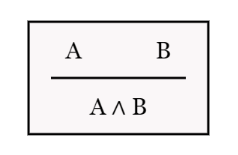
\includegraphics[scale=0.5]{2Top1Bottom}} \\
\hline
1 Top / 1 Bottom &  [``A $\wedge$ B", ``\%", `` B", ``\%"] & \raisebox{-.5\height}{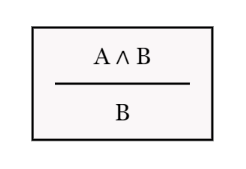
\includegraphics[scale=0.5]{1Top1Bottom}} \\
\hline
\end{tabular}
\end{center}

When dots are represented in the proof, the ID number of the dot number is the element in the proof structure. The drawing algorithm will recognise a number and render it in a dot. The ID numbers of the dot will link to a dot and the dot object with the position coordinates associated with it.

The way larger proof trees were stored was in the form of nested lists. If an element of the list is stored as another list, then a proof structure of the same format can be contained there. This system works recursively to create proofs in tree shapes, which can then be easily be drawn by the software.

Proofs with dots and multiple layered proofs are represented as follows:

\begin{center}
\begin{tabular}{ |c|p{4.5cm}|c| } 
\hline
Dots in a proof &  [1, 2, 3, ``\%"] & \raisebox{-.5\height}{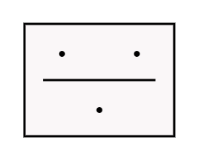
\includegraphics[scale=0.5]{dots}} \\
\hline
Multi-line Proof &  [[``A", ``B", ``A $\wedge$ B", ``\%"], ``C", ``(A  $\wedge$ B) $\wedge$ C"] & \raisebox{-.5\height}{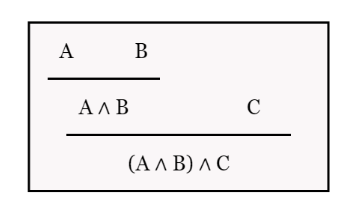
\includegraphics[scale=0.5]{multiline}} \\
\hline
\end{tabular}
\end{center}

A simple, unified proof system allows both ease when drawing and when assessing the proof to check whether it is valid. Because the structure is consistant, comparison is possible.

\section{Unification Algorithm}

An important requirement for this software project was to recognise whether a proof is valid and correct. In Natural Deduction logic you can't automatically use distributive, associative or communicative properties automatically. \cite{intro} Every proof needs to be shown explicitly. This means that Natural deduction proofs can only be reordered where the substance of every branch is the same, but the location in the proof can be different.

As as simple example consider A $\wedge$ B. Having both A and B on the top line states that A is true and B is true. Whether the A is on the left or the B is on the left is irrelevent but this shows that proofs can be represented differently. A whole proof tree can look very different whilst representing the same proof logically and this project provides an algorithm that achieves this.

\centerline{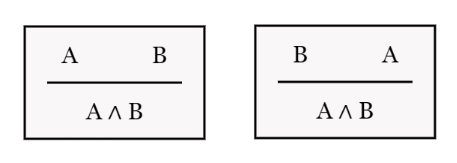
\includegraphics[scale=0.5]{unification}}

 The key part to this algorithm is that is uses recursion. The algorithm makes sure that a branch of the tree matches a branch of one, ideal solution that is provided. If this branch is correct then other branches are checked, again by recursion. If all branches in the user's answer are accounted for and match up with the ideal answer given then the solution is valid. If any one of the branches doesn't match up then the proof is obviously incorrect. It will return that the user's proof is incorrect and allow the user to try again.

By having this generic algorithm in place, it makes the system very flexible. Adding levels is incredibly easy because only one valid proof needs to be submitted and then all of the valid solutions will be permitted. This makes the software both flexible and easily scalable which are another two key requirements for this software. 

\section{Drawing and rendering algorithms}

The drawing algorithm is another important part of the software to make sure that the proof is presented to the user in the way that they expect. Presenting information to the user correctly and reliably is a key feature that this project much achieve. The drawing algorithm uses setInterval which is a javascript function that runs a function at certain intervals. This runs the drawing algorithm that redraws what is on the canvas, giving a user an instant reaction to whatever moves they are performing.

The drawing algorithm was written in a way that it interprets the data structure to correctly render the proof in a tree shape. The drawing algorithm takes into account whether each structure is ``2 Top/1 Bottom" or ``1 Top/1 Bottom" and draws it appropriately. It also takes into account any dots in the system, which are represented as numbers in the proof system. The algorithm realises these numbers and renders them as a dot to the user. 

Multi level proofs need to drawn in a different location because they are on top of the first level of structure. Because of the potential different proof widths that need to be drawn, the first 4 levels of proof are individually accounted for. If more that four levels of proof need to be drawn, a recursive function is used. Another box linking to the proof is drawn in the same format as the original proof. This is done for ease of readibility. The user will still be able to read all parts of the proof easily.

In retrospect, a better drawing function could and should be created. One that offers the whole proof in one object that is still readable would be ideal. An algorithm that uses recursion more would reduce repetitive code. Tree like structures lend themselves well to recursion, so this could have been utilised more. 

One feature that does work well is the resizing of boxes. When the height of a proof is increased, the size of the box will automatically increase as well. As the height increases, the width will also increase proportionally as well. This is to make sure that items on the top row on the proof will still be rendered clearly and that the user has a good user experience.

\section{Levels and how the Software was turned into a Game}

Although making sure the mathematic logic was complete and works successfully, it is just as important for this project to come across as a game to the user. There are many tools already available that will aid a user in learning Natural Deduction, but as previously discussed, many of these do not engage the user and lack other key elements that make these tools into games. Part of the implementation of this project was putting in key gamification attributes that would make this tool a game.

One of the main features that was important to include was the concept of levels. The implementation of levels in this game restricts the user from using certain elements and this helps the user by guiding them in what buttons they can press. In the Figure below, which represents Level 1 of the software, only the buttons needed to create A $\wedge$ B are eligable to press. Buttons unavailable are greyed out and when the user hovers the mouse over the button, a 'not allowed' symbol is displayed.  

\centerline{
\includegraphics[scale=0.65]{buttons}}

Free play offers the user all of the buttons available but has no end goal for the user. A user can still drag and drop everything but the proof cannot be compared to anything. Clicking to check the proof runs the unification algorithm previously mentioned. This will either end the level and start the next one if the user is correct. If the user is wrong, it will let them try again.

The penalty for letting the user trying again is a reduction in a game score. A user gets score of 10 for every level successfully completed with no mistakes. Every mistake they make- that is when they click 'Check Proof' and the proof is incorrect- is a deduction of two points. A user successfully completing a level correctly will always receive 1 point, no matter how many attempts are taken. Scores for all the levels are accumilated and a final score for a user is given.

The user can then play the game again and although it will be the same levels, the user can keep trying until they get a perfect score of 10 for every level. This makes the game more replayable and will hopefully subconciously solidify the knowledge the user is learning about Natural Deduction. Scoring adds a competitive element between friends as well. Beating a peer may mean that a user has to play through the game again to get a better score, all of which will increase learning when the user plays through the game again.

By using levels and a scoring system, instant feedback can be relayed to the user. The user will know if there proof is correct as soon as they are ready. This gives the user feedback on demand when they want it. As well as this, further help can be provided via a hints button that has been implemented. This is to aid the user in the learning process. Clicking the hints button reduces the score by 2 points, so it encourages the user not to use the hints, but they are available if needed.
